\documentclass[a4paper,11pt]{report}

/stock/16_git_repo/library/library.tex

\begin{document}
% Page de garde <<<
../../../../00_resources/page_garde.tex
% >>>

\chapter{Introduction}

La théorie de l'ordonnancement est une branche ancienne et fondamentale de l'informatique, ayant
pour objectif d'organiser et de répartir un ensemble de travaux entre les différents actifs. Ayant
un lien direct avec l'organisation et la gestion de projets, l'ordonnancement n'est pas une notion
nouvelle. En effet, des constructions telles que les pyramides d'Égypte où les aqueducs romains
n'auraient pu voir le jour sans aucune forme d'orodonnancement.

Cependant les premières traces de formalisme, posant les bases de l'ordonnancement tel que nous
le connaissons, ont été introduites par Joseph Priestley~\cite{joseph_priestley_description_1764}
sous la forme d'un diagramme proche d'un frise chronologique en 1764. Puis il faut attendre 1896,
pour voir apparaître l'\emph{Harmonogram}, connu actuellement sous le nom de diagramme de Gantt,
décrit par l'économiste polonais Karol Adamiecki. Malheureusement, les écrits de ce dernier, publiés
dans se langue maternelle, ne se démocratisent pas en occident, et c'est donc Henry Gantt, ingénieur
américain, qui publie une description de ces diagrammes en 1910.

C'est en 1959, lors d'une conférence, que James Kelley et Morgan Walker~\cite{kelley1959critical}
présentent le premier algorithme d'ordonnancement appelé \emph{Critical Path Method}, ouvrant la
porte au développement de la théorie de l'ordonnancement.

Des problématiques aussi diverses que la planification de prises de photographies par satellite,
l'agencement spatial de marchandises dans un entrepôt ou la planification d'une chaîne de production
peuvent être modélisées par des problèmes d'ordonanncement comme en témoigne la longue liste
d'articles et de livres détaillant nombre de déclinaisons de problèmes
considérés comme classiques. Cette étude bibliographique, préliminaire au stage, s'inscrit dans cette
démarche et cherche à définir le contexte et les bases nécessaires à l'introduction d'une variante
d'un problème d'ordonnancement très étudié que l'on appelle \isched{}.

\section{Description des problèmes d'ordonnancement}

Nous utiliserons au cours de cette partie les notations communément utilisées pour définir de
manière générale les problèmes d'ordonnancement. Nous serons amenés à définir et utiliser des
notations plus spécifiques au problème considéré.

D'ordinaire, les problèmes d'ordonnancement sont définis par un ensemble de $n$ tâches $\mathcal{T} =
\{T_1, T_2, \dots, T_n\}$ et par un ensemble de $m$ machines\footnote{On les appelle aussi des
processeurs.} $\mathcal{M} = \{M_1, M_2, \dots, M_m\}$. L'ordonnancement consiste à affecter les
tâches $\mathcal{T}$ aux machines $\mathcal{M}$ tout en respectant les contraintes définies par
le problème initial. On peut citer trois contraintes largement répandues dans la théorie de
l'ordonnancement :
\begin{enumerate}
    \item chaque machine peut exécuter au plus une seule tâche à tout instant,
    \item chaque tâche est exécutée par au plus une machine,
    \item chaque tâche est exécutée par au moins une machine.
\end{enumerate}
Un ordonnancement est dit valide, s'il respecte l'ensembles des contraintes imposées.

Il paraît important de notifier, qu'il existe des problèmes autorisant l'exécution d'une tâche sur
plusieurs machines, la durée d'exécution de la tâche est alors proportionnelle au nombre de
machines sur lesquelles elle s'exécute. On parle alors de modèles hiérarchiques, mais ces modèles
ne seront pas développés dans le reste de ce manuscrit.

\section{Caractérisation des machines}

Dans le but de décrire un problème d'ordonnancement, il est important de définir l'environnement des
machines, c'est à dire les hypothèses considérées sur ces dernières. Au cours de ce rapport, seul
le modèle des machines parallèles, exécutant toutes les mêmes fonctions, sera considéré. Pour la
découverte du modèle des machines dédiées, spécialisées dans l'exécution de certaines fonctions,
nous invitons les intéressés à la lecture du livre~\cite{blazewicz_handbook_2007}.

Les machines parallèles se décomposent en trois catégories :
\begin{enumerate}
    \item identiques : tous les machines de $\mathcal{P}$ admettent la même vitesse de traitement
    \item uniformes : les vitesses de traitement diffèrent mais la vitesse de traitement est
        proportionnelle à un coefficient propre à chaque machine appelé facteur d'accélération
    \item générales : les vitesses de traitement dépendent des tâches à effectuer
\end{enumerate}

À nouveau nous ne considérerons qu'une seule catégorie, les problèmes nous intéressant ne portent
que sur des machines identiques.

\section{Caractérisation des tâches}

Généralement, en ordonnancement, une tâche est définie par cinq paramètres :
\begin{enumerate}
    \item un vecteur de temps d'exécution $p_j = ^t(p_{j1}, p_{j2}, \dots, p_{jm})$ où $p_{ji}$
        représente le temps nécessaire à l'exécution de la tâche $T_j$ sur la machine $i$. Dans le cas
        de machines identiques et uniformes, une tâche s'exécute à la même vitesse sur toutes les
        machines, $p_j$ se réduit alors à un réel,
    \item une date de disponibilité $r_j$, désignant la date à partir de laquelle la tâche est prête
        à être exécutée,
    \item une date d'échéance $d_j$, désignant la date souhaitée à laquelle la tâche $T_j$ devrait
        être exécutée,
    \item une date de fin impérative $\widetilde{d_j}$, date à laquelle la tâche doit
        obligatoirement être exécutée. Contrairement à la date d'échéance souhaitée, si une tâche
        finit son exécution après sa date de fin impérative, l'ordonnancement produit n'est pas
        valide,
    \item un poids $w_j$, représentant l'urgence relative de la tâche.
\end{enumerate}


\section{Contraintes sur les tâches}

Il est possible de définir des contraintes sur les tâches, modifiant leur ordre ou encore  leur
mode d'exécution. Les contraintes de précédence permettent d'imposer un ordre d'exécution entre deux
tâches $T_i$ et $T_j$ : $T_i \prec T_j$ signifie que la tâche $T_j$ ne peut être exécutée qui si
$T_i$ a fini son exécution. Ces contraintes peuvent être représentées par un graphe orienté associant un
sommet à chaque tâche et tel qu'il existe une arc allant d'un sommet $u$ à un sommet $v$ si et
seulement si la tâche associée à $u$ précéde celle associée à $v$. Ce graphe est appelé graphe de
précédence, et s'il ne possède aucun arc, alors les tâches sont indépendantes.

Des contraintes peuvent aussi être imposées à l'ensemble de tâches par l'intermédiaire d'un graphe
relatif à ces dernières, que nous appellerons le graphe d'exclusion, qui à chaque tâche associe
un sommet, et tel qu'il existe une arête entre deux sommets si deux taches ne peuvent être affectée
à la même machine, il est alors possible d'imposer des contraintes structurelles à ce graphe. 

On peut, par exemple, imposer à ce graphe d'être un graphe d'intervalles. Un graphe d'intervalles
est un graphe tel que ses sommets sont représentables par des intervalles et il existe une arête
entre deux sommets si et seulement si les intervalles associés à ces sommets s'intersectent
lorsqu'ils sont représentés sur la ligne des réels. Un exemple de graphe d'intervalles est donné à la
figure~\ref{fig:ex_gint}. 

Les problèmes d'ordonnancement tels que le graphe d'exclusion est un graphe d'intervalles définissent une
sous-branche de l'ordonnancement appelée \isched{} que nous décrirons plus loin.

\begin{figure}
    \centering
    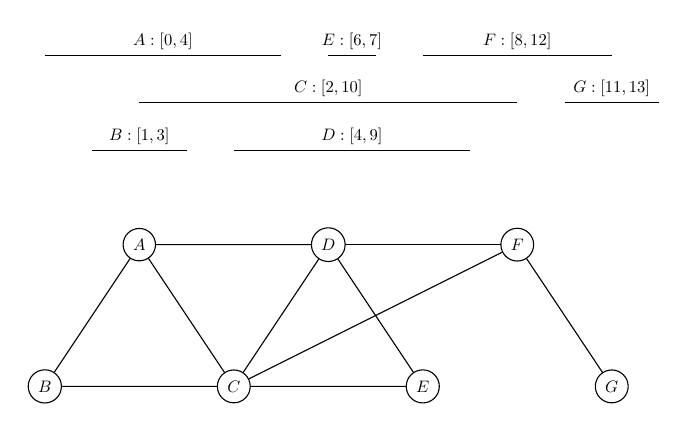
\begin{tikzpicture}[noeud/.style={draw=black, circle}, scale=0.6, every node/.style={transform shape}]
        \draw[-] (0,  0) to node[above] {$A : [0,4]$} (5,0);
        \draw[-] (1, -2) to node[above] {$B : [1,3]$} (3,-2);
        \draw[-] (2, -1) to node[above] {$C : [2, 10]$} (10, -1);
        \draw[-] (4, -2) to node[above] {$D : [4, 9]$} (9, -2);
        \draw[-] (6,  0) to node[above] {$E : [6,7]$} (7,0);
        \draw[-] (8,  0) to node[above] {$F : [8,12]$} (12,0);
        \draw[-] (11, -1) to node[above] {$G : [11, 13]$} (13, -1);

        \node[noeud] (A) at (2, -4) {$A$};
        \node[noeud] (B) at (0, -7) {$B$};
        \node[noeud] (C) at (4, -7) {$C$};
        \node[noeud] (D) at (6, -4) {$D$};
        \node[noeud] (E) at (8, -7) {$E$};
        \node[noeud] (F) at (10, -4) {$F$};
        \node[noeud] (G) at (12, -7) {$G$};

        \draw[-] (A) to (B);
        \draw[-] (A) to (C);
        \draw[-] (A) to (D);

        \draw[-] (B) to (C);
        
        \draw[-] (C) to (D);
        \draw[-] (C) to (E);
        \draw[-] (C) to (F);

        \draw[-] (D) to (E);
        \draw[-] (D) to (F);

        \draw[-] (F) to (G);
    \end{tikzpicture}
    \caption{Un exemple de graphe d'intervalles}
    \label{fig:ex_gint}
\end{figure}

\section{Notation à trois champs}

La multitude de problèmes d'ordonnancement énoncée précédemment a conduit à la mise en place d'une
notation synthétique permettant la description de ces schémas. Nous nous proposons de reprendre la
notation introduite par Graham~\cite{graham} et B\l a\.zewicz~\cite{blazewicz}. 

Pour cette notation, il nous faut introduire trois paramètres $\alpha, \beta, \gamma$. Détaillons
ces paramètres :
\begin{enumerate}
    \item le paramètre $\alpha$ permet de caractériser l'environnement des machines. $\alpha \in
        \left\{ P, \bar{P}, P_m, \right\}$, avec :
        \begin{itemize}
            \item \textcolor{red}{$P$} : les machines sont identiques et leur nombre est une entrée du
                problème, 
            \item $\bar{P}$ : les machines sont identiques, mais leur nombre est dit suffisant ou
                non borné,
            \item $P_m$ : les machines sont identiques et leur nombre est fixé,
        \end{itemize}
        $P$ est l'environnement de machines que nous utiliserons par la suite.
    \item le paramètre $\beta$ permet de définir le type d'application et ses caractéristiques
        telles que les contraintes de précédence ou les durées d'exécution des tâches. Nous écrirons
        ce paramètre sous la forme $\beta = \beta_1\beta_2\beta_3$ avec :
        \begin{itemize}[label=$\bullet$]
            \item $\beta_1$ représentant les contraintes de précédence :
                \begin{itemize}
                    \item $\beta_1 = prec$ : le graphe de précédence est un graphe quelconque
                    \item $\beta_1 = arbre$ : le graphe de précédence est un arbre
                    \item[$\vdots$]
                    \item $\beta_1 = .$ : les tâches sont indépendantes
                \end{itemize}
            \item $\beta_2$ représentant les temps d'exécution des tâches :
                \begin{itemize}
                    \item $\beta_2 = p_j = 1$ : les tâches sont unitaires, leur durée est égale à
                        $1$
                    \item $\beta_2 = .$ : les durées des tâches sont données par le graphe
                \end{itemize}
            \item $\beta_3$ représentant les propriétés structurelles du graphe d'exclusion :
                \begin{itemize}
                    \item \textbf{$\beta_3 = intervalle$} : le graphe d'exclusion est un graphe d'intervalles
                    \item $\beta_3 = .$ : le graphe d'exclusion est un graphe vide (sans arêtes)
                \end{itemize}
        \end{itemize}
    \item le paramètre $\gamma$ représente quant à lui définit la fonction objectif que l'on
        cherchera à optimiser. Il existe plusieurs fonctions objectifs qui sont communément
        utilisées en ordonnancement classique, nous introduisons brièvement deux d'entre elles :
        \begin{itemize}
            \item $C_{max}$ : cette fonction a pour objectif de minimiser le temps total d'exécution,
                appelé \emph{makespan}, étant égal à la différence entre le début et la fin de
                l'exécution de l'ensemble des tâches,
            \item $\sum w_j c_j$ : cette fonction permet de prendre en compte l'urgence relative des
                tâches en minimisant la somme des produits du temps de compéltion par l'urgence
                relative.
        \end{itemize}
\end{enumerate}

\section{Motivations}

% TODO: Étoffer
Les problèmes considérés tout au long de ce rapport s'inscrivent dans la branche de l'ordonnancement
appelée \isched{}, dans cette branche le début et la fin de chaque tâche $T_j$ sont
fixés, la tâche est donc représentable par un intervalle $\left[ \st{j}, \ct{j} \right]$ et un poids
$w_j$, et toutes les tâches ne sont pas obligatoirement exécutées.

La possibilité de ne pas exécuter certaines tâches entraîne l'établissement de nouvelles fonctions
objectif, les fonctions relatives au temps d'exécution ayant un intérêt moindre, pour ne pas dire
nul\footnote{$C_{max}$ est, par exemple, systématiquement optimale pour un ordonnancement
vide(n'exécutant aucune tâche).}. Parmis ces fonctions, nous citerons celles de maximisation du
profit généré par l'exécution des tâches ou de maximisation du nombre de tâches exécutées toutes
deux introduites plus précisément au cours de l'état de l'art. 

Il est
usuel, lorsque l'on travaille avec ce genre de fonctions, de considérer un ensemble de tâches tel
qu'il est impossible de pouvoir assigner à chaque tâche une machine : intuitivement, un
ordonnancement affectant une machine à chaque tâche est un ordonnancement optimal. Or nous verrons
au cours de la section suivante, que trouver un tel ordonnancement se fait en temps polynomial à
l'aide, par exemple d'algorithmes de flots~\cite{arkin_scheduling_1987}.

%Intuitivement, on conçoit que la difficulté des problèmes d'ordonnancement pour lesquels les dates
%de débuts des tâches ne sont pas fixées repose sur leur grand nombre d'ordonnancements valides.
%En effet, étant donnée une machine et $3$ tâches, il existe $6$ ordonnancements différents valides
%ou invalides. En étendant le problème à $n$ tâches, il est possible de décrire $n!$ ordonnancements
%différents.  Dans l'\isched{}, peut importe le nombre de tâches à affecter à une seule et unique
%machine, il existe un seul ordonnancement possible qui de surcroît peut être invalide. De manière
%plus formelle, 

%Un grand nombre de fonctions objectif définies pour l'ordonnancement classique présentent un
%intérêt moindre pour l'\isched{} : la fonction $C_{max}$ est en effet constante lorsque les dates de
%début et de fin d'exécution de chacune des tâches sont fixées. C'est pourquoi de nouvelles fonctions
%ont été introduites telles que la maximisation du profit généré par l'exécution des tâches. 

Le but de ce stage est d'étudier une nouvelle fonction objectif pour ces problèmes cherchant à
optimiser la flexibilité de l'ordonnancement produit en minimisant la fragmentation de celui-ci. La
mesure choisie portera sur ce que nous appellerons les trous désignant le temps de repos d'une
machine entre deux tâches qui lui sont affectées. Elle repose sur un constat simple : plus la période
d'inactivité d'une machine est grande, plus celle-ci sera à même de traiter de nouvelles tâches;
autrement dit, en cherchant à obtenir de longues périodes d'inactivité pour chacune des machines, on
augmente le nombre de tâches susceptibles d'être acceptées ultérieurement et donc la flexibilité de
l'ordonnancement obtenu.


\newpage
\chapter{État de l'art}


Cette section se propose d'exhiber une infime partie des problèmes relatifs à l'ordonnancement
ainsi que quelques solutions proposées pour résoudre ceux-ci. Nous présenterons, dans un premier
temps, le problème \bisched{} ainsi qu'un certain nombre de résultats sur ce dernier. Puis nous
introduirons quelques unes des nombreuses variantes de ce problème et là aussi nous décrirons
quelques résultats que l'on peut trouver dans la littérature. Ces problèmes ont été choisis pour les
similitudes qu'ils présentent avec le problème étudié.

\section{Le problème \bisched{}}

Étant donnés un ensemble de $n$ tâches $\mathcal{T} = \left\{
T_1, T_2, \dots, T_n \right\}$ représentés par un ensemble de $n$ intervalles $\mathcal{I} = \{
[ \st{T_1}, \ct{T_1} ], [ \st{T_2}, \ct{T_2} ], \dots, [ \st{T_n},
\ct{T_n} ] \}$ avec $\ct{T_i} > \st{T_i}$ pour $i = 1, \dots, n$, et un ensemble de
machines $\mathcal{M} = \left\{ M_1, M_2, \dots, M_m \right\}$, le but est alors de trouver un
ordonnancement minimisant le nombre de machines utilisées par ce dernier.

On peut définir la notation à trois champs de ce problème :
\begin{center}
    $\bar{P} \Big| p_j, intervalle \Big| \min \#(\mathcal{M})$
\end{center}

Le problème \bisched{} a été démontré équivalent à la recherche du nombre chromatique du graphe d'intervalle
associé au problème~\cite{golumbicalgorithmic}. Le nombre chromatique d'un graphe étant le plus
petit nombre de couleurs nécessaires à la coloration d'un graphe. Dans la mesure où le problème de
coloration de graphes d'intervalles est polynomiale, le problème \bisched{} l'est aussi, ainsi Ford et
Fulkerson ont proposé en 1962, un algorithme s'exécutant en $O(n^2)$
opérations~\cite{ford1962network}. Depuis d'autres méthodes ont été proposées notamment par Gupta et
al.~\cite{gupta_optimal_1978} ayant une complexité en $O(n\log n)$ opérations.

L'algorithme repose sur une observation simple : le nombre minimal de couleurs nécessaires à la
coloration du graphe d'intervalle est égal à la taille de la plus grande clique de ce graphe, or une
clique de taille $k$ dans le graphe associé à l'ensemble des tâches correspond à une durée pendant
laquelle $k$ intervalles s'intersectent deux à deux. Ainsi, en parcourant les dates de début des tâches par
ordre de dates de début, et en assignant cette tâche à une machine, ayant déjà été utilisée
précédemment, l'algorithme s'assure qu'une nouvella machine est utilisée lorsque le nombre de
tâches s'intersectant deux à deux est supérieur aux nombres de machines déjà utilisées. Dans ce cas
le nombre de couleurs déjà utilisées pour colorer le graphe est inférieur à la taille de la clique
courante (et donc nécessairement de la plus grande clique).

Un algorithme distribué a été mis au point par Dekel et Sani~\cite{dekel1983parallel}, permettant la
résolution de ce problème en $O(\log n)$ moyennant $O(n^2 / \log n)$ machines.

\section{Quelques variantes}

Il existe beaucoup de déclinaisons du problème \bisched{} considérant une autre fonction objectif,
modifiant l'environnement des machines, ou encore introduisant de nouvelles notions permettant
d'augmenter l'expressivité du modèle. Parmi ces variantes, nous en avons choisi deux permettant de
définir le contexte de notre modèle.

\subsection{Nombre de machines fixé}

Cette variante, contrairement au problème originel, fixe le nombre de machines pouvant exécuter les
tâches et cherche un ordonnancement permettant de maximiser la somme du poids des tâches affectées à
une machine. Le poids $w_j$ d'une tâche $T_j$ peut être vu comme le profit généré par l'exécution de
la tâche $T_j$, le problème cherche alors à maximiser les gains.

Nous noterons ce problème :
\begin{center}
    $P \Big| p_j, intervalle \Big| \max \sum w_j : j$ est affectée à une machine de $\mathcal{M}$
\end{center}

Sans contraintes supplémentaires, le problème est polynomial, Arkin et Silverberg ayant proposé en
1986 un algorithme s'exécutant en $O(n^2 \log n)$ opérations~\cite{arkin_scheduling_1987}. Cet
algorithme repose sur la même observation que celui de Gupta et al.~\cite{gupta_optimal_1978} précédemment présenté : il faut
exactement $p$ couleurs pour colorer une clique de taille $p$. Donc étant donné $\mathcal{M}=\left\{
M_1, M_2, \dots, M_m \right\}$ un ensemble de $m$ machines, pour toutes les cliques de taille
$p$ supérieure à $m$, l'algorithme cherche à supprimer les $p - m$ sommets de la clique présentant
le plus petit profit. Ces sommets sont identifiés à l'aide d'un algorithme de flot de coût minimum
dans un graphe construit à partir des cliques du graphes d'intervalles de départ.

Cet algorithme a donc la particularité de trouver un ordonnancement de profit maximal, non pas en
trouvant les tâches à affecter, mais en trouvant celle à ne pas affecter.

À présent, considérons ce même problème, à ceci prêt : chaque tâche $T_j$ de $\mathcal{T}$ va se voir
attribuer un ensemble de machines $\mathcal{M}_j \subseteq \mathcal{M}$ représentant l'ensemble des
machines sur lesquelles la tâche $T_j$ peut être exécutée.

Ce problème devient alors \npc si le nombre de machine dans chaque sous-ensemble $\mathcal{M}_j$ est
supérieur ou égal à $3$~\cite{arkin_scheduling_1987}, la preuve se faisant par une réduction depuis
le problème \textsc{$3-$SAT}. Un algorithme exprimé sous forme de programmation dynamique a été
décrit dans ce même article, il s'exécute en $O(n^{k+1})$.

Bhatia et al.~\cite{bhatia2003algorithmic} ont proposé une $(1 - 1/\varepsilon)-$approximation
randomisée, dont une partie de l'exécution repose sur des données aléatoires, basée sur de la
programmation linéaire permettant la résolution de ce problème. De plus de nombreuses heuristiques
ont été introduite pour répondre à ce problème, nous renvoyons les intéressés à la lectures des
articles~\cite{kroon1995exact} et~\cite{gabrel1995scheduling}.

\subsection{Indisponibilité de machines}

Une seconde extension au problème \bisched{} est une variante introduisant des périodes au cours
desquelles certaines machines seront dites indisponibles et donc pendant lesquelles elles ne
pourront effectuer aucun calcul. La machine entrant en indisponibilité ne doit avoir aucune tâche en
court d'exécution, un ordonnancement présentant une intersection entre une tâche et une
indisponibilité n'est donc pas un ordonnancement valide.

Comme vu précédemment, les problèmes d'ordonnancement d'intervalles ont un lien fort avec les
graphes d'intervalles, \bisched{} étant équivalent au problème de coloration sur ces derniers. Il
existe une catégorie de graphe, à savoir les graphes à arcs circulaires qui est le
graphe d'intersection d'un ensemble d'arcs de cercle, dont le problème de coloration est équivalent
au problème avec machines indisponibles. Un exemple de graphe est donné à la figure~\ref{fig:ex_ac}.

Le problème \isma{} a été démontré \npc par
Papadimitriou~\cite{papadimitriou1982private} à l'aide d'une réduction depuis le problème de
coloration sur un graphe à arcs circulaires. La réduction inverse, depuis \isma{} vers le problème de
coloration, a été décrite plus tard par Kolen et al.~\cite{kolen2007interval}. Ces mêmes auteurs ont également
proposé deux algorithmes exacts pour la résolution de ce problème, le premier utilise la
programmation dynamique s'exécutant en $O(ln^{l+1})$, avec $l$ la taille de la plus grand clique dans
le graphe à arcs circulaires. Le second algorithme, quant à lui, réalise une énumération  basée sur
la notion d'ordonnancement partiel : un ordonnancement partiel jusqu'à la date $t$ est une
assignation à une machine de chacune des tâches dont la date de début est antérieure à $t$ de sorte
que deux tâches de s'exécutent en même temps sur la même machine. Cette algorithme s'exécute en
$O\left( n+k \right)k!k \log k)$ opérations, avec $k$ le nombre de machines. Cet algorithme est
particulièrement intéressant puisque si le nombre de machines pour \isma{} est fixé, alors l'algorithme
devient linéaire en le nombre de tâches.

\begin{figure}
    \centering
    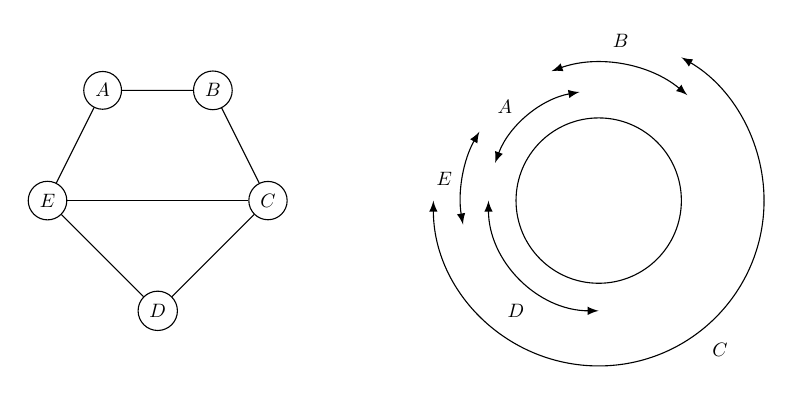
\begin{tikzpicture}[n/.style={draw=black, circle}, scale=0.7, every node/.style={transform shape}, >=latex]
        \node[n] (A) at (1, 4) {$A$};
        \node[n] (B) at (3, 4) {$B$};
        \node[n] (C) at (4, 2) {$C$};
        \node[n] (D) at (2, 0) {$D$};
        \node[n] (E) at (0, 2) {$E$};

        \draw[-] (A) to (B);
        \draw[-] (A) to (E);

        \draw[-] (B) to (C);

        \draw[-] (C) to (D);
        \draw[-] (C) to (E);

        \draw[-] (D) to (E);

        \draw (10,2) circle (1.5cm);
        \draw[rotate around={100:(10,2)}, <->] (12, 2) arc (0:60:2cm);
        \draw[rotate around={150:(10,2)}, <->] (12.5, 2) arc (0:40:2.5cm);
        \draw[rotate around={180:(10,2)}, <->] (12, 2) arc (0:90:2cm);
        \draw[rotate around={180:(10,2)}, <->] (13, 2) arc (0:240:3cm);
        \draw[rotate around={ 50:(10,2)}, <->] (12.5, 2) arc (0:60:2.5cm);

        \node (a) at (8.3, 3.7) {$A$}; 
        \node (b) at (10.4, 4.9) {$B$}; 
        \node (c) at (12.2, -0.7) {$C$}; 
        \node (d) at (8.5, 0) {$D$}; 
        \node (e) at (7.2, 2.4) {$E$}; 
        
    \end{tikzpicture}
    \caption{Exemple de graphe à arcs circulaires}
    \label{fig:ex_ac}
\end{figure}

Il existe différentes façons de représenter l'indisponibilité d'une machine pendant une période
donnée. Supposons que nous ayons une machine $M$ indisponible pendant le laps de temps représenté par
l'intervalle $i_M = \left[ \sint{i_M}, \cint{i_M} \right]$, une première façon d'envisager un tel
scénario est de considérer deux machines $M_1, M_2$ telles que la machine $M_1$ est disponible
pendant la durée $\left[ 0, \sint{i_M} \right]$ et la machine $M_2$ est disponible entre les dates
$\left[ \cint{i_M}, \infty \right]$. Une seconde façon de voir ce scénario est de considérer que
l'indisponibilité de la machine n'est autre qu'une tâche préaffectée à la machine indisponible. C'est
cette représentation que nous allons utiliser pour l'introduction du problème \fisched{} qui sera
étudié tout au long de ce stage.

\subsection{Flexibilité de l'ordonnancement}

Nous introduisons la notion de flexibilité d'un ordonnancement décrivant
sa capacité à pouvoir accepter un plus grand nombre de tâches ultérieurement. L'origine de cette
problématique est due à l'accroissement de services proposés par les grandes compagnies numériques
sur la toile. Il est en effet possible, de louer les ressources de calcul générées par une machine
pendant une durée définie par l'utilisateur. La question visant à maximiser le profit ayant été
largement étudiée, nous nous intéressons à la manière d'ordonnancer les tâches à disposition afin de
pouvoir garantir l'acceptation de toute tâche répondant à une contrainte. 

Pour mesurer la flexibilité de l'ordonnancement nous avons fait le choix d'introduire la notion de
trou : un période d'inactivité non nulle d'une machine délimitée à gauche et à droite par des tâches
ordonnancées sur la dite machine. Il paraît en effet évident qu'un trou de grande longueur sera
susceptible d'accueillir un plus grand nombre de tâches futures qu'une multitude de petit trous.
La fonction objectif considérée cherchera donc à maximiser le plus petit des trous de
l'ordonnancement produit.

Enfin, nous plaçons dans un contexte tel que les machines ne sont pas continûment disponible: nous
considérons un ensemble de tâches préaffectées à un ensemble de machines, représentant les tâches
ayant été précédemment ordonnancées. Ces périodes d'inactivités
seront appelées réservations, et dorénavant, les trous considérés pourront être délimités à gauche
et à droite par des tâches et/ou des réservations.

Si l'on considère :
\begin{itemize}
    \item $\mathcal{T} = \left\{ T_1, T_2, \dots, T_n \right\}$, l'ensemble des tâches à ordonnancer
        associé à un ensemble d'intervalles $\mathcal{I} = \left\{ i_{T_1}, i_{T_2}, \dots,
        i_{T_n} \right\}$,
    \item $\mathcal{M} = \left\{ M_1, M_2, \dots, M_m \right\}$ l'ensemble des machines 
    \item $\mathcal{R} = \left\{ l_1, l_2, \dots, l_h \right\}$ l'ensemble des réservations
        représentable par un couple $\left( M_l, \left[ \sres{l}, \cres{l} \right] \right)$
        comprenant la machine à laquelle est préaffectée la réservation $l$ et l'intervalle
        représentant la période d'indisponibilité de la machine $M_l$
    \item $H_{\min} = \min \left\{ \sint{i'} - \cint{i} > 0 : i, i' \in \mathcal{T} \cup
        \mathcal{R} \right\}$ la fonction permettant de calculer la valeur du trou minimum,
\end{itemize}
alors la notation à trois champs de notre problème est la suivante :
\begin{center}
    $P \Big| p_j, intervalle \Big| \max H_{\min}$
\end{center}

\newpage

\chapter{Travaux à mener}

Le stage portant sur le problème précédemment introduit sera abordé de la manière suivante :
\begin{enumerate}
    \item Dans un premier temps, nous nous intéresserons à la classification du problème du point de
        vue de la complexité classique : \fisched{} est-il \npc? Et du point de vue de la complexité
        paramétrée : est il FPT?
    \item Puis nous chercherons à mettre au point différents algorithmes exacts ou
        d'approximation\footnote{Uniquement si le problème est \npc.} avec garantie de performances.
        Les techniques porteront sur la formulation du problème en programmation linéaire en nombre
        entier et sur la programmation dynamique.
    \item Enfin nous envisagerons différentes variantes du problème telles qu'une variante online,
        l'ensemble des tâches à ordonnancer est alors initialement inconnu ou connu en partie
        seulement, les autres tâches sont dévoilées au fur et à mesure du temps, qui paraît
        s'inscrire naturellement dans le sillage de notre problème.
\end{enumerate}

\newpage
\appendix
\bibliographystyle{plain}
\bibliography{biblio}


\end{document}
